%!TEX root = ../../book_ML.tex
\chapter{Quá khớp}
\label{cha:overfitting}

\index{quá khớp -- overfitting}
\index{overfitting -- quá khớp}

\textit{Quá khớp} (overfitting) là một hiện tượng không mong muốn thường gặp, người xây dựng mô hình
machine learning cần nắm được các kỹ thuật để tránh hiện tượng này.

\section{Giới thiệu}
% \index{tính phổ quágeneralization}

Trong các mô hình học có giám sát, ta thường
phải đi tìm một mô hình ánh xạ các vector đặc trưng thành các kết quả tương ứng
trong tập huấn luyện. Nói cách khác, ta cần đi tìm hàm số $f$ sao cho $y_i \approx f(\bx_i),
~\forall i = 1, 2,
\dots, N$. Một cách tự nhiên, ta sẽ đi tìm các tham số mô hình của $f$ sao cho
việc xấp xỉ có sai số càng nhỏ càng tốt. Điều này nghĩa là mô hình càng
\textit{khớp} với dữ liệu càng tốt. Tuy nhiên, sự thật là nếu một mô hình {quá
khớp} với dữ liệu huấn luyện thì nó sẽ gây phản tác dụng. Quá khớp là một hiện tượng không mong muốn mà người xây dựng mô hình machine learning cần lưu ý.
Hiện tượng này xảy ra khi mô hình tìm được mang lại kết quả cao trên tập huấn
luyện nhưng không có kết quả tốt trên tập kiểm tra. Nói cách khác, mô hình tìm được không có tính tổng quát.

Để có cái nhìn đầu tiên về quá khớp, chúng ta cùng xem ví dụ trong
Hình~\ref{fig:15_polyreg}. Có 50 cặp điểm dữ liệu ở đó đầu ra là một đa thức bậc
ba của đầu vào cộng thêm nhiễu. Tập dữ liệu này được chia làm hai phần: tập huấn luyện gồm 30 điểm
dữ liệu hình tròn, tập kiểm tra gồm 20 điểm dữ liệu hình vuông. Đồ thị của đa thức bậc ba này được cho bởi đường nét đứt. Bài toán đặt ra là hãy tìm
một mô hình tốt để mô tả quan hệ giữa đầu vào và đầu ra của dữ liệu đã cho. Giả sử thêm rằng đầu ra xấp xỉ là một đa thức của đầu vào.


Với $N$ cặp điểm dữ liệu $(x_1, y_1), \dots, (x_N, y_N)$ với các $x_i$ khác nhau
đôi một, luôn tìm được một {đa thức nội suy Lagrange} $P(x)$ bậc không
vượt quá $N-1$ sao cho $P(x_i) = y_i, ~\forall i = 1, 2, \dots, N$.


\begin{figure}[t]
\begin{subfigure}{0.49\textwidth}
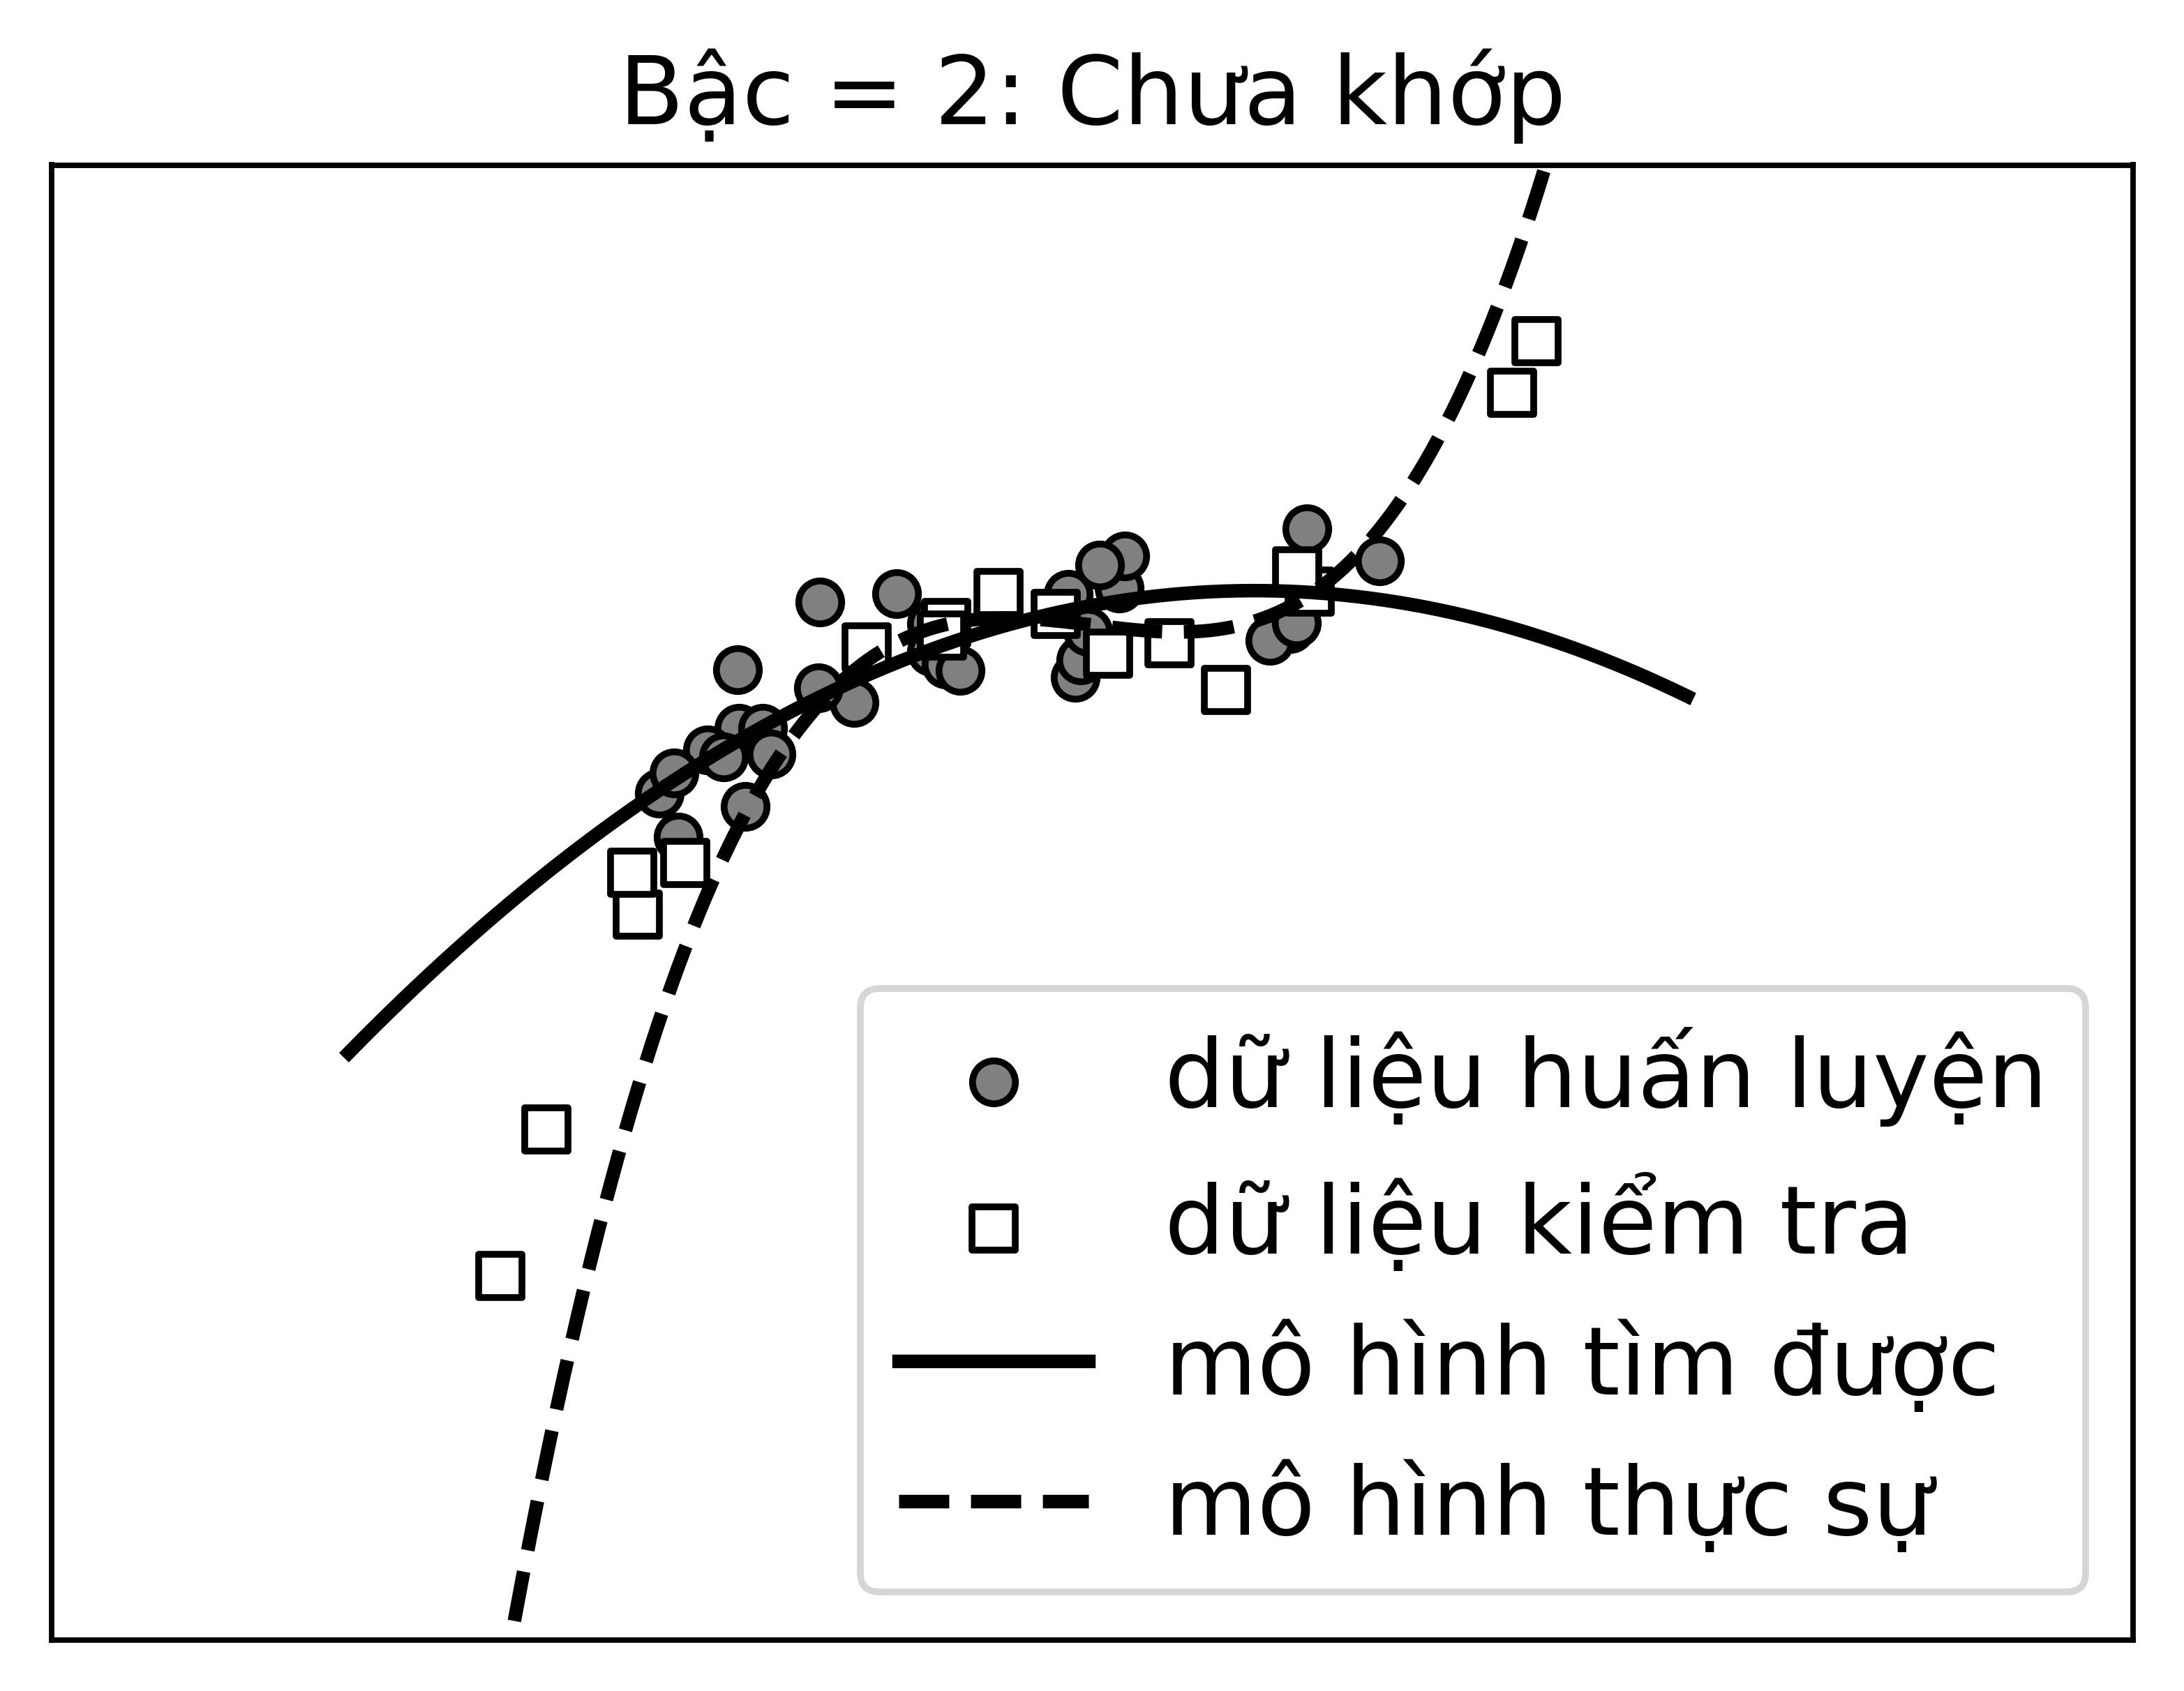
\includegraphics[width=0.99\linewidth]{ebookML_src/src/overfitting/poly2.png}
% {Chapters/01_Overview/15_overfitting/linreg_2.png}
\caption{}
\label{fig:15_polyrega}
\end{subfigure}
\begin{subfigure}{0.49\textwidth}
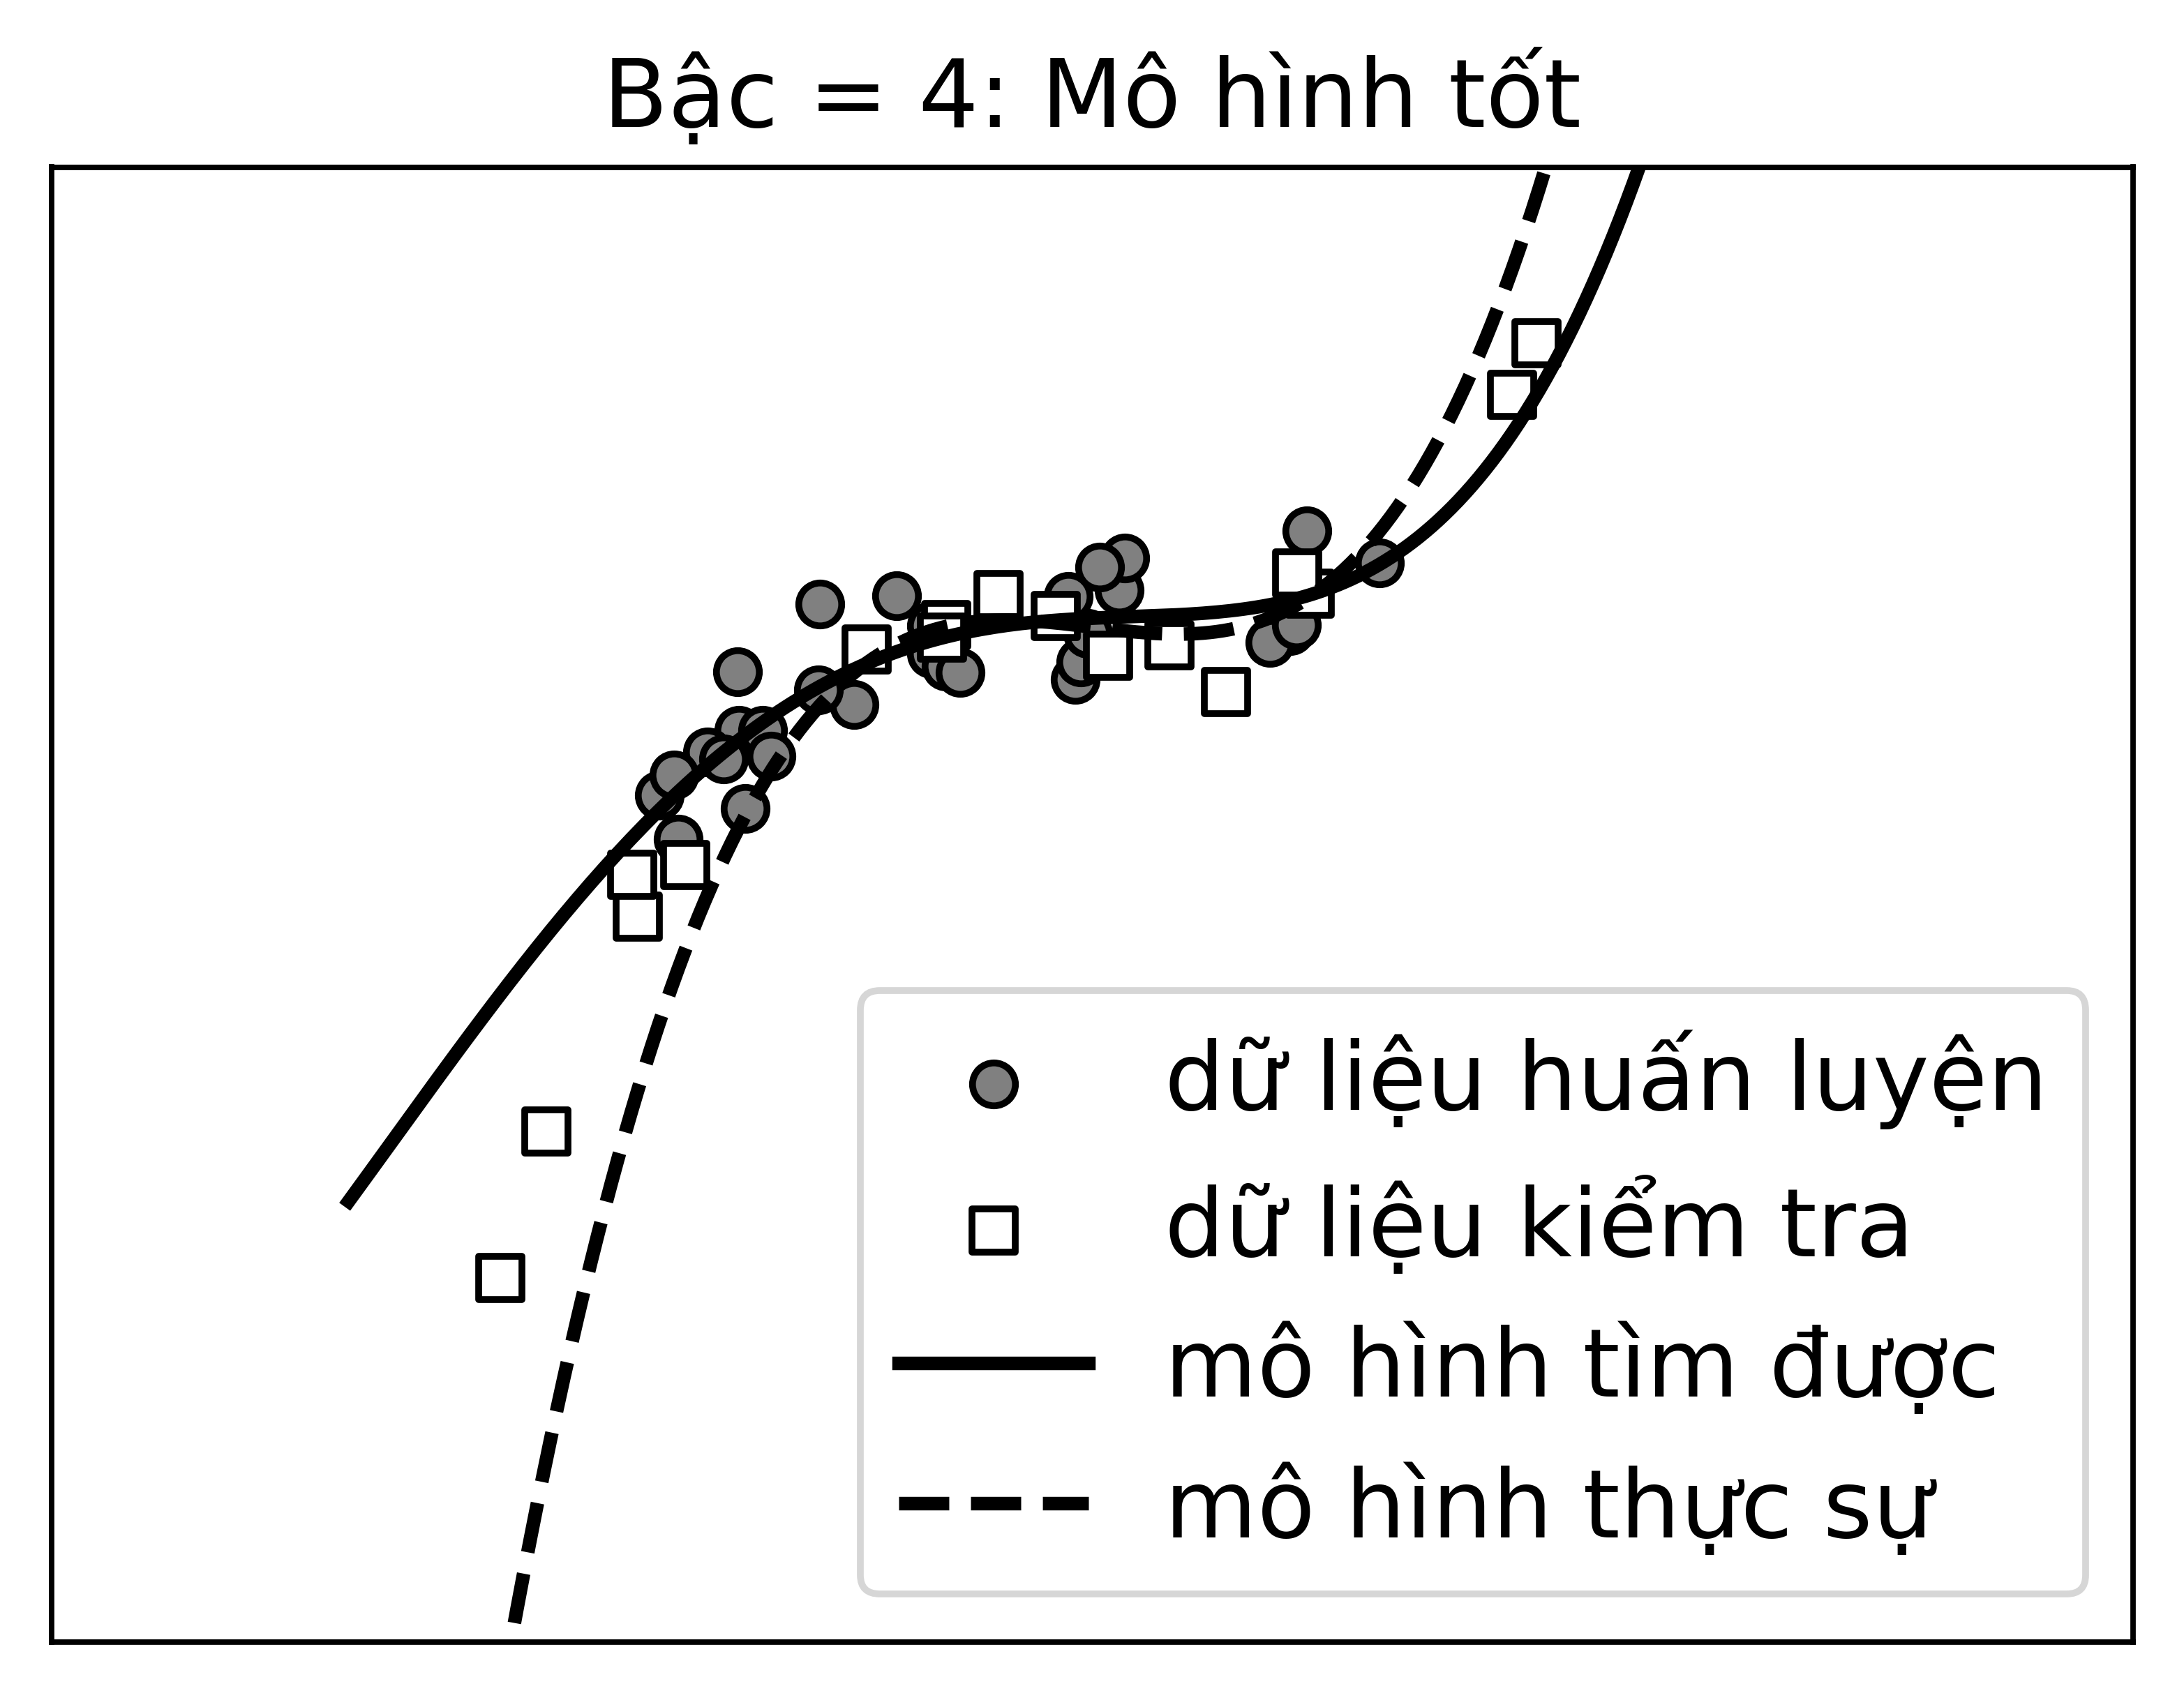
\includegraphics[width=0.99\linewidth]{ebookML_src/src/overfitting/poly4.png}
% {Chapters/01_Overview/15_overfitting/linreg_4.png}
\caption{}
\label{fig:15_polyregb}
\end{subfigure}
\begin{subfigure}{0.49\textwidth}
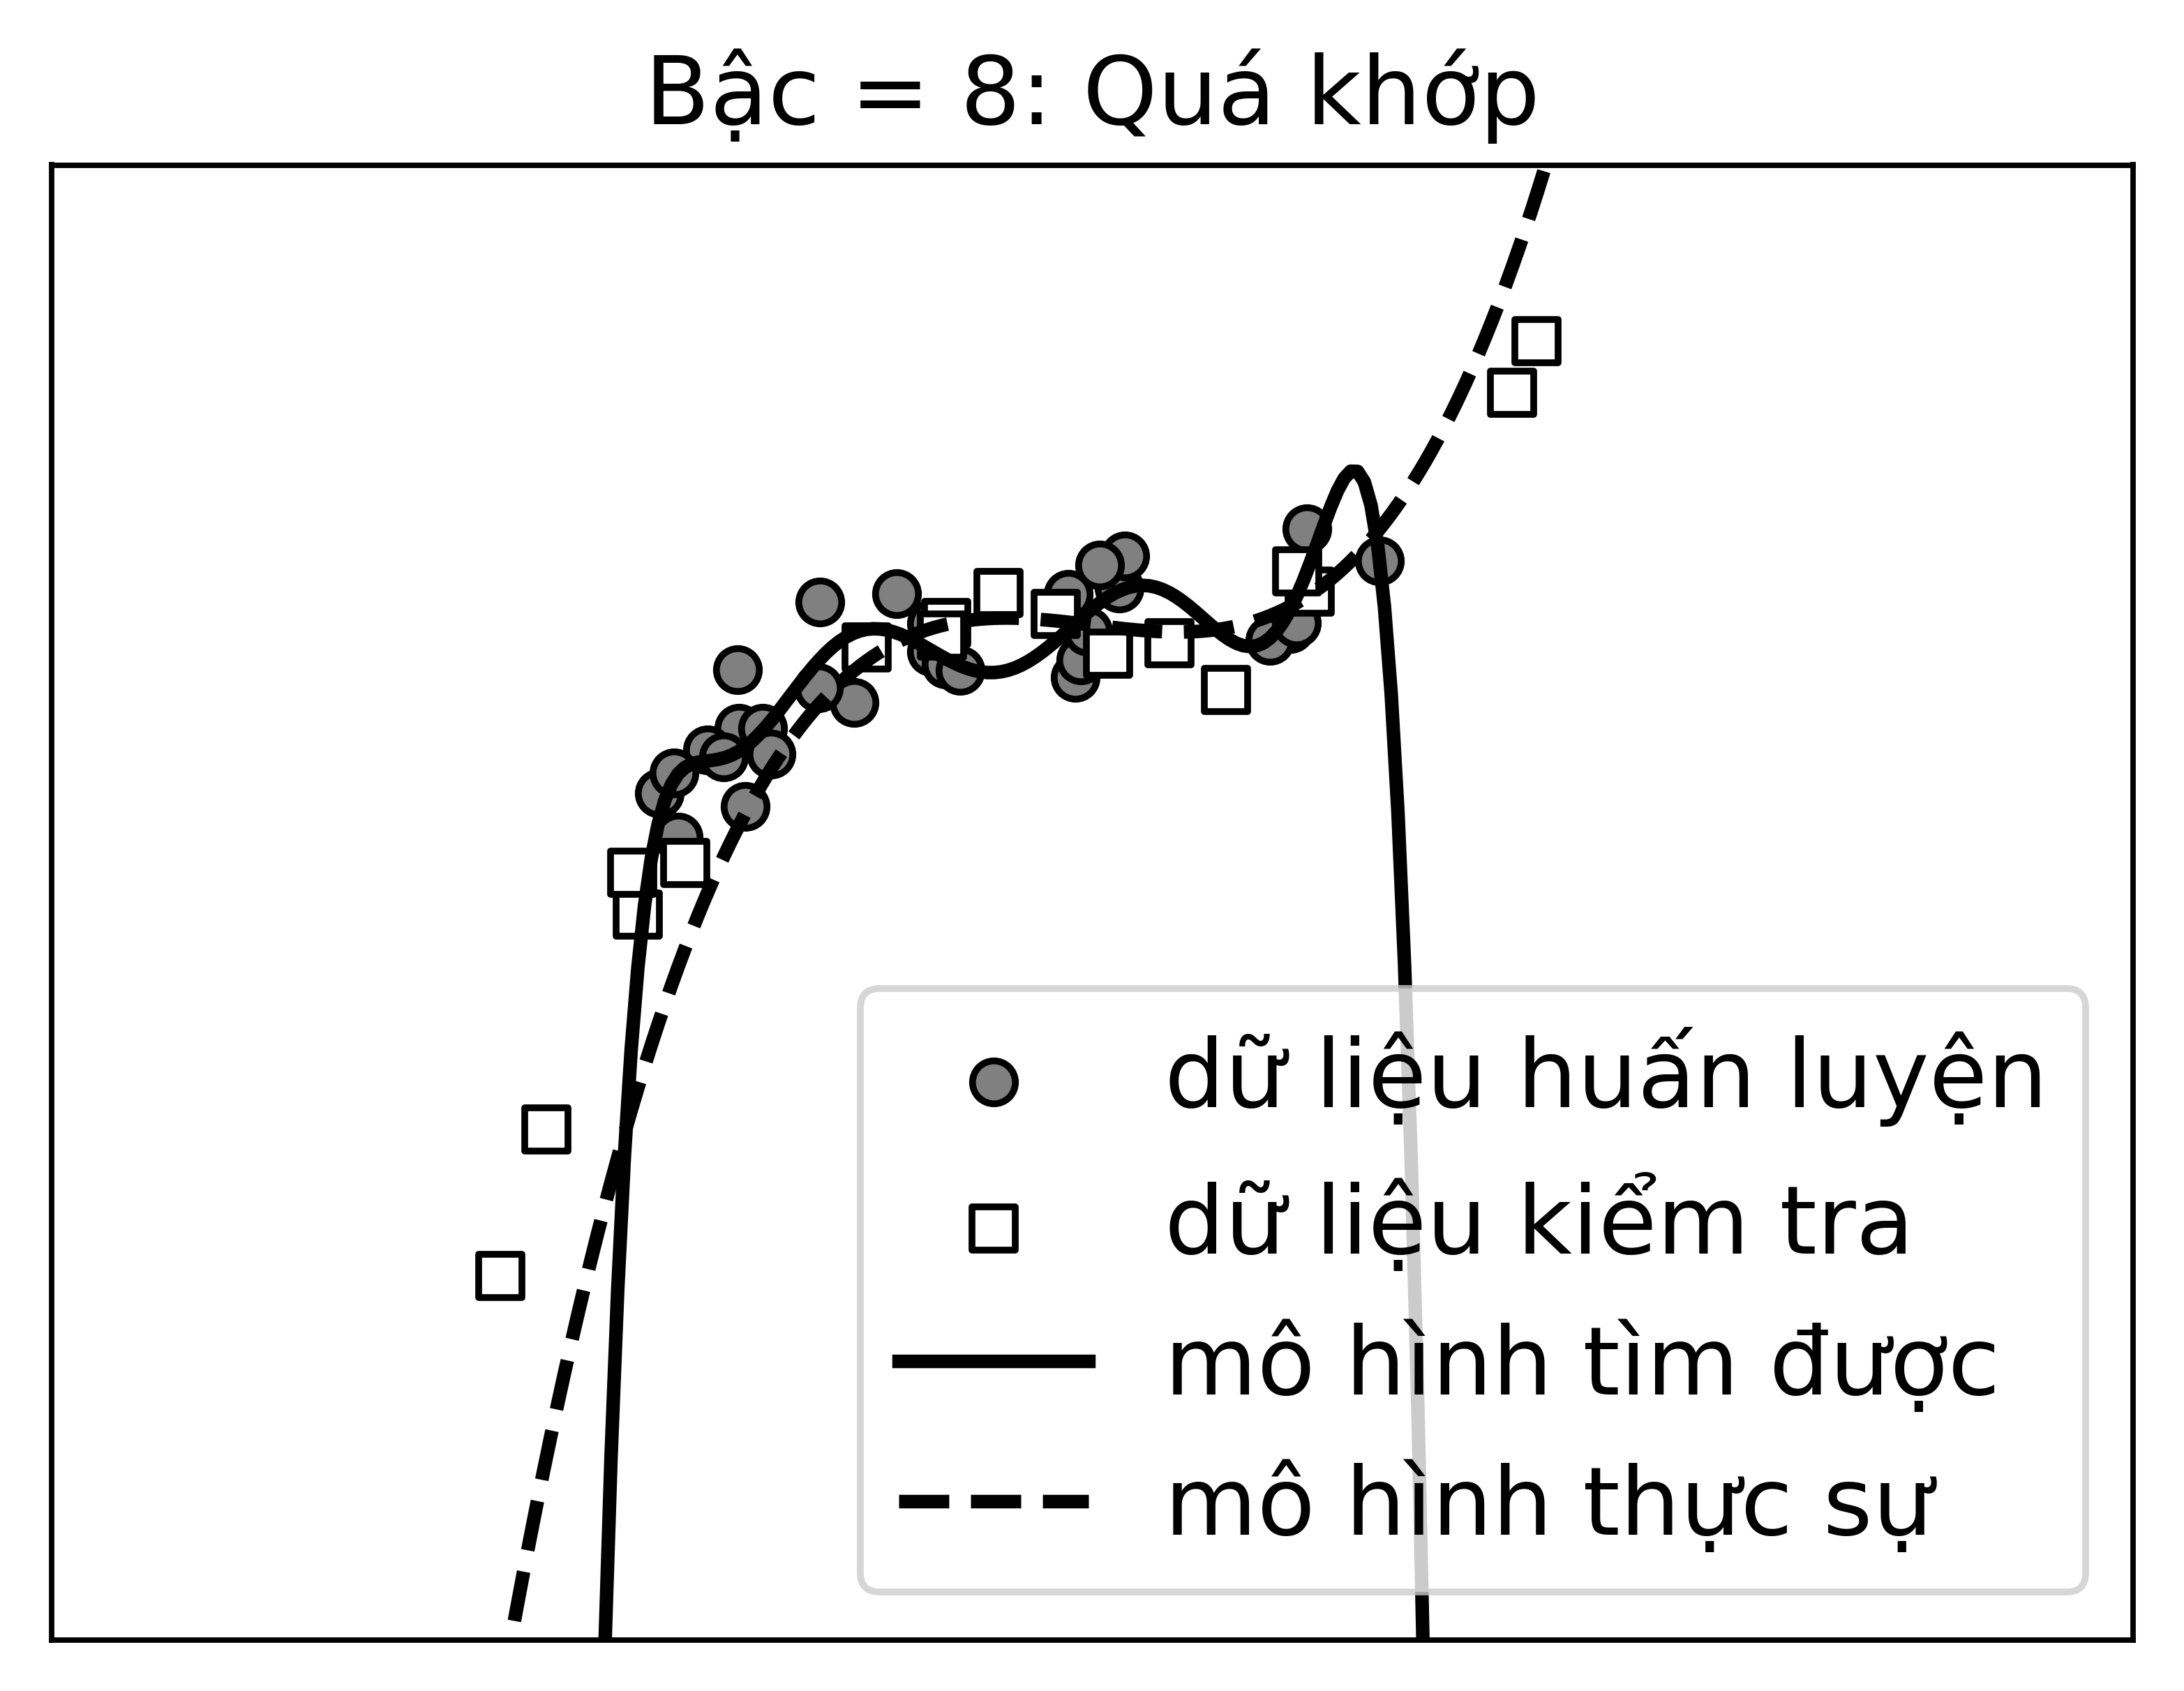
\includegraphics[width=0.99\linewidth]{ebookML_src/src/overfitting/poly8.png}
% {Chapters/01_Overview/15_overfitting/linreg_8.png}
\caption{}
\label{fig:15_polyregc}
\end{subfigure}
\begin{subfigure}{0.49\textwidth}
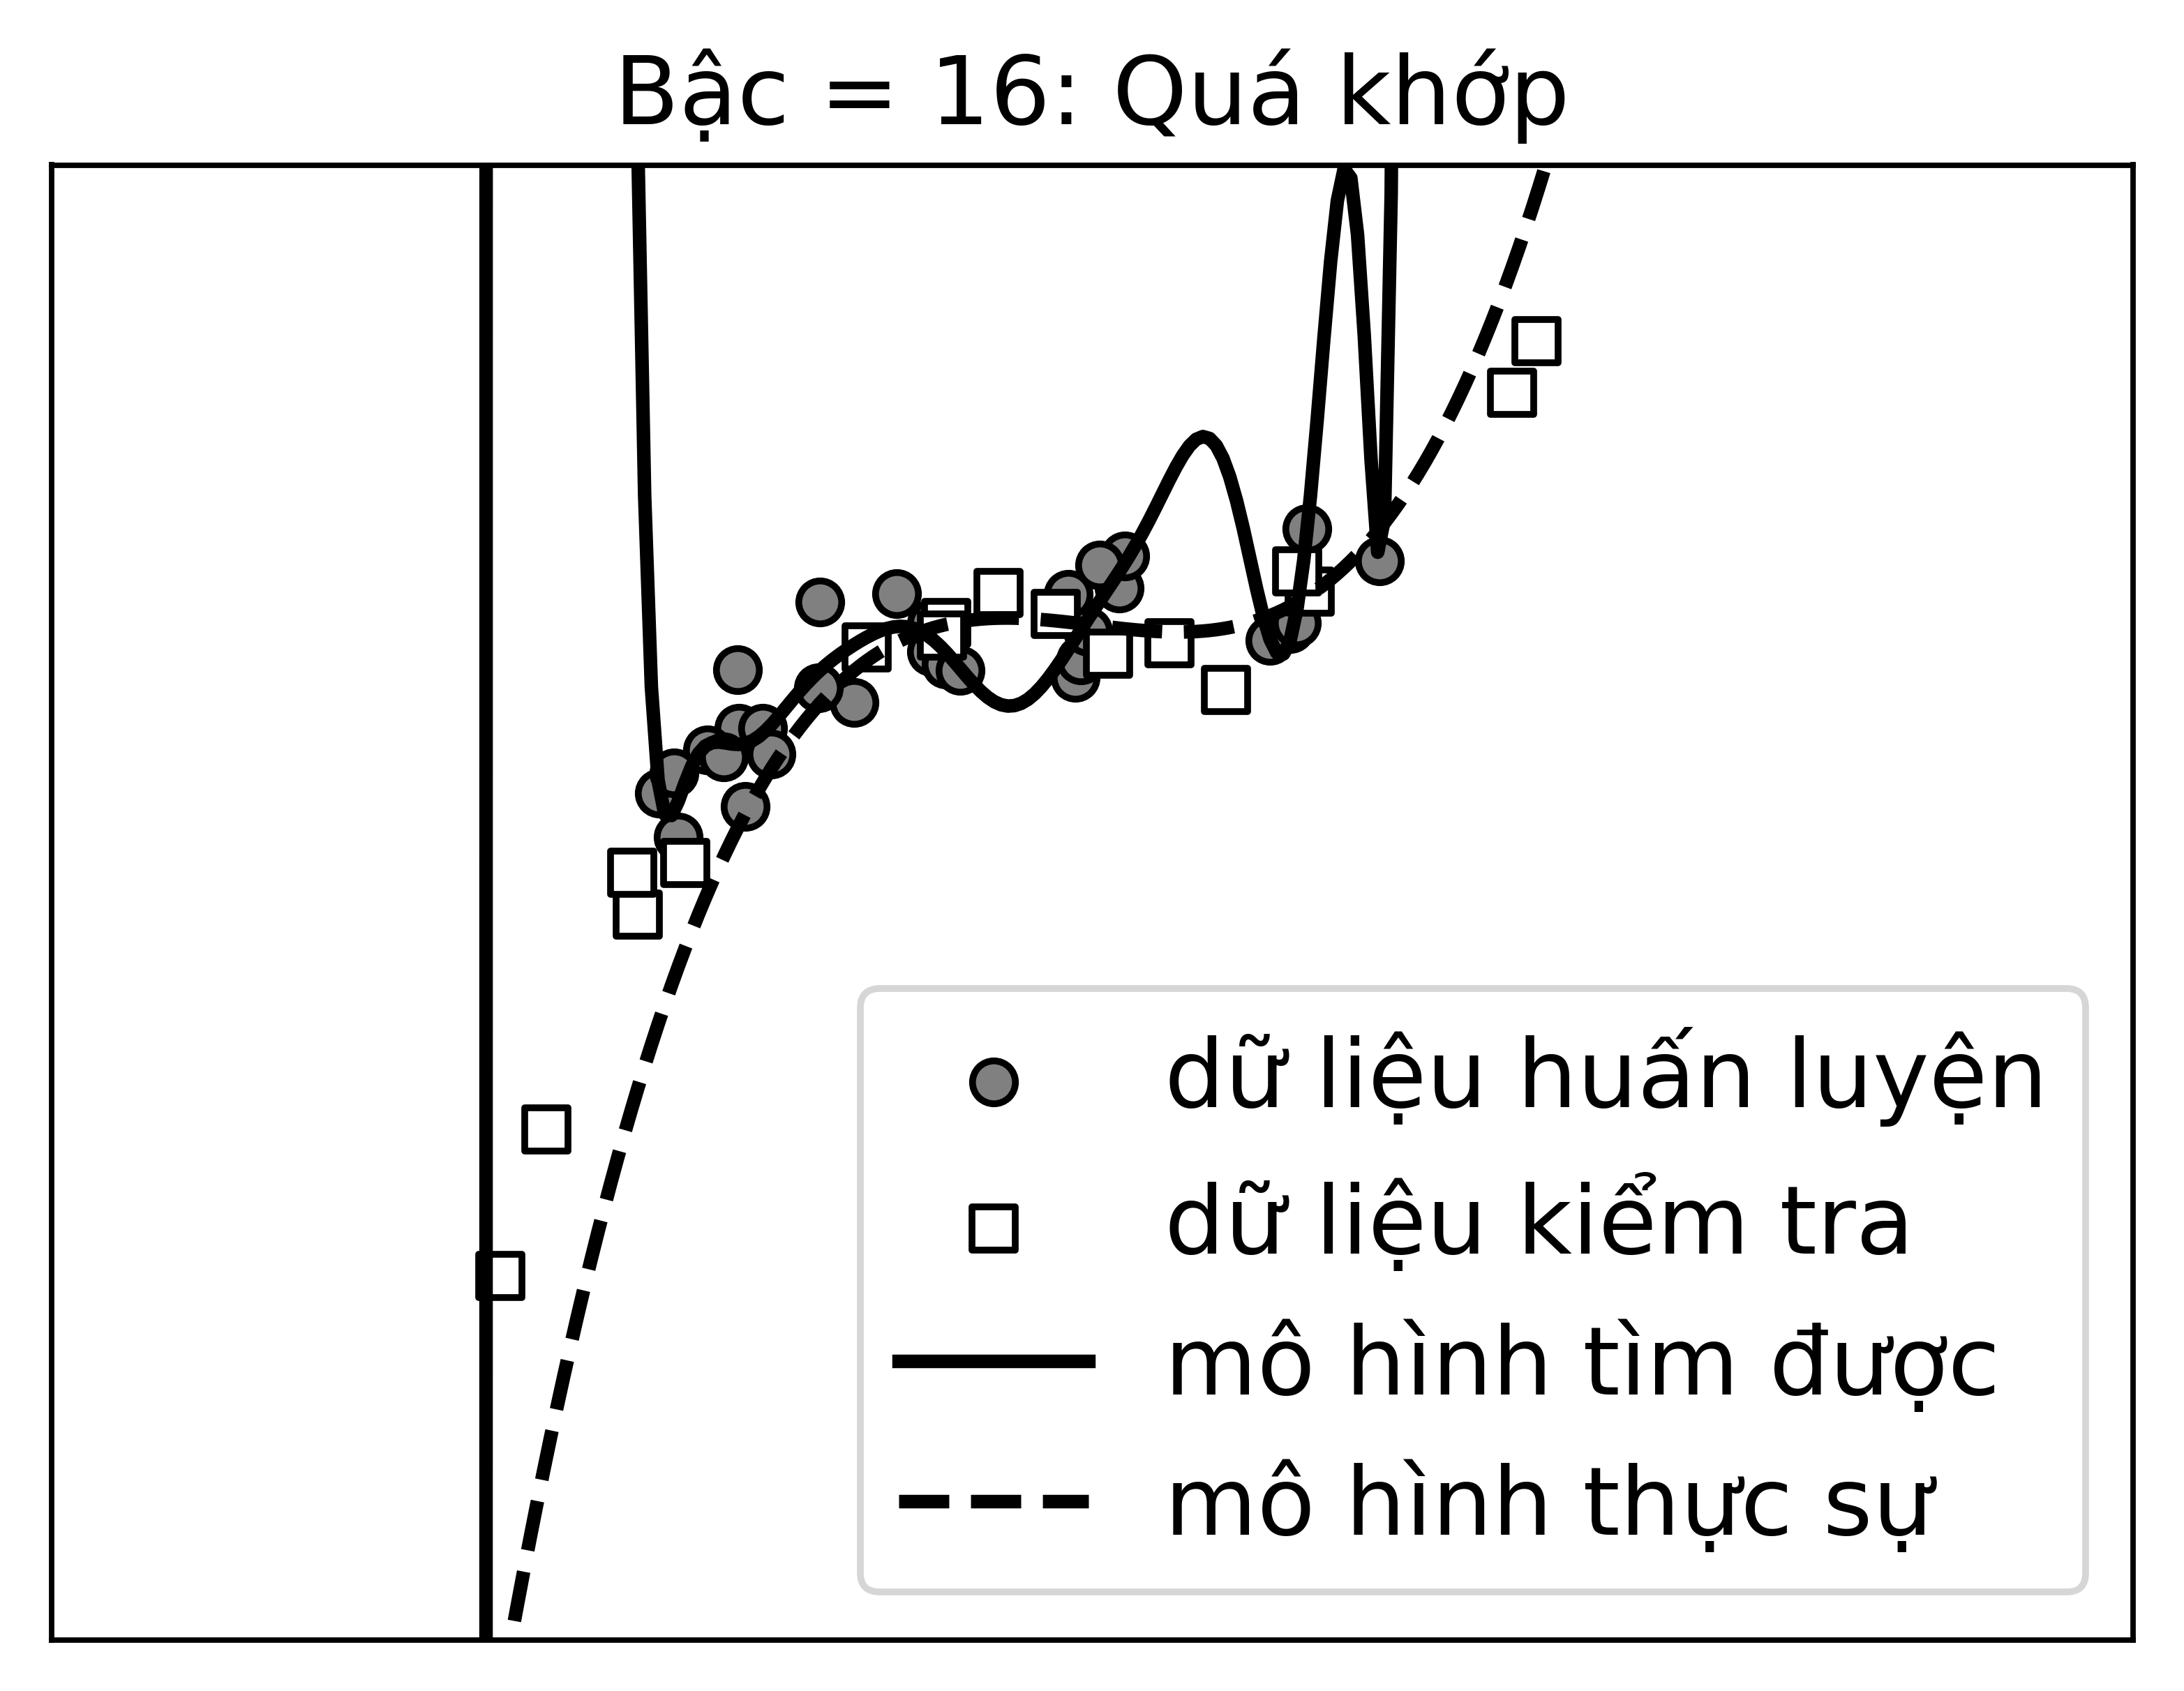
\includegraphics[width=0.99\linewidth]{ebookML_src/src/overfitting/poly16.png}
% {Chapters/01_Overview/15_overfitting/linreg_16.png}
\caption{}
\label{fig:15_polyregd}
\end{subfigure}
\caption{
Chưa khớp và quá khớp trong hồi quy đa thức.
}
\label{fig:15_polyreg}
\end{figure}

Như đã đề cập trong Chương~\ref{cha:linear_regression}, với loại dữ liệu này,
chúng ta có thể áp dụng hồi quy đa thức với vector đặc trưng
$\mathbf{x} = [1, x, x^2, x^3, \dots, x^d]^T$ cho đa thức bậc $d$. Điều quan
trọng là cần xác định bậc $d$ của đa thức. Giá trị $d$ còn được gọi là siêu tham số của mô hình.

\index{hồi quy đa thức -- polynomial regression}
\index{polynomial regression -- hồi quy đa thức}
\index{chưa khớp -- underfitting}
\index{underfitting -- chưa khớp}
Rõ ràng một đa thức bậc không vượt quá 29 có thể mô tả chính xác dữ liệu huấn
luyện. Tuy nhiên, ta sẽ xem xét các đa thức bậc thấp hơn $d = 2, 4, 8, 16$. Với
$d = 2$, mô hình không thực sự tốt vì mô hình dự đoán (đường nét liền) quá khác
so với {mô hình thực}; thậm chí nó có xu hướng đi xuống khi dữ liệu đang
có hướng đi lên. Trong trường hợp này, ta nói mô hình bị \textit{chưa khớp} (underfitting).
Khi $d = 8$, với các điểm dữ liệu trong tập huấn luyện, mô hình dự đoán và mô
hình thực khá giống nhau. Tuy nhiên, đa thức bậc 8 cho kết quả hoàn toàn ngược
với {xu hướng của dữ liệu} ở phía phải. Điều tương tự xảy ra trong trường hợp $d
= 16$. Đa thức bậc 16 này quá khớp với tập huấn luyện. Việc quá khớp
trong trường hợp bậc 16 là không tốt vì mô hình có thể đang cố gắng mô tả
{nhiễu} thay vì dữ liệu. Hiện tượng xảy ra ở hai trường hợp đa thức bậc
cao này chính là quá khớp. Độ phức tạp của đồ thị trong hai
trường hợp này cũng khá lớn, dẫn đến các đường dự đoán không được tự nhiên. Khi bậc của đa thức tăng lên, độ phức tạp của nó cũng tăng theo và hiện tượng quá khớp xảy ra nghiêm trọng hơn.

% \textit{Nếu bạn nào biết về Đa thức nội suy Lagrange thì có thể hiểu được hiện tượng sai số lớn với các điểm nằm ngoài khoảng của các điểm đã cho. Đó chính là lý do phương pháp đó có từ "nội suy", với các trường hợp "ngoại suy", kết quả thường không chính xác.}

Với $d = 4$, mô hình dự đoán khá giống với mô hình thực. Hệ số bậc cao nhất tìm
được rất gần với 0\footnote{Mã nguồn tại \url{https://goo.gl/uD9hm1}.}, vì
vậy đa thức bậc bốn này khá gần với đa thức bậc ba ban đầu. Đây chính là một mô
hình tốt.


Quá khớp sẽ gây ra hậu quả lớn nếu trong tập huấn luyện có nhiễu. Khi
đó, mô hình quá chú trọng vào việc bắt chước tập huấn luyện mà quên đi việc
quan trọng hơn là tính tổng quát. Quá khớp đặc biệt xảy ra khi lượng dữ liệu huấn
luyện quá nhỏ hoặc độ phức tạp của mô hình quá cao. Trong ví dụ trên đây, độ
phức tạp của mô hình có thể được coi là bậc của đa thức cần tìm.

% Trong
% \href{http://machinelearningcoban.com/2017/02/24/mlp/}{Multi-layer Perceptron},
% độ phức tạp của mô hình có thể được coi là số lượng hidden layers và số lượng
% units trong các hidden layers.

Vậy, có những kỹ thuật nào giúp tránh quá khớp?

Trước hết, chúng ta cần một vài đại lượng để đánh giá chất lượng của mô hình
trên tập huấn luyện và tập kiểm tra. Dưới đây là hai đại lượng đơn giản, với
giả sử $\mathbf{y}$ là đầu ra thực sự, và $\mathbf{\hat{y}}$ là đầu ra dự đoán
của mô hình. Ở đây, đầu ra có thể là một vector.

\index{sai số huấn luyện}
\index{sai số trung bình bình phương -- mean squared error, MSE}
\index{mean squared error, MSE -- sai số trung bình bình phương}
\textbf{Sai số huấn luyện} (training error): Đại lượng này là mức độ sai khác giữa đầu ra thực và đầu
ra dự đoán của mô hình. Trong nhiều trường hợp, giá trị này chính là hàm mất mát khi áp dụng lên dữ liệu huấn luyện. Hàm mất mát này cần có một thừa số $\displaystyle
\frac{1}{N_{\text{train}}}$ để tính giá trị trung bình mất mát
trên mỗi điểm dữ liệu. Với các bài toán hồi quy, đại lượng này thường được xác định bởi \textit{sai số trung bình bình phương} ({mean squared error -- MSE}):
\begin{equation*}
\text{sai số huấn luyện}= \frac{1}{2N_{\text{train}}} \sum_{\text{tập huấn luyện}}
\|\mathbf{y} - \mathbf{\hat{y}}\|_2^2
\end{equation*}
% với $p$ \href{http://machinelearningcoban.com/math/#mot-so-chuan-thuong-dung}{thường bằng 1 hoặc 2}.
Với các bài toán phân loại, có nhiều cách đánh giá mô hình trên các tập dữ liệu. Chúng ta sẽ dần thấy trong các chương sau.

\textbf{Sai số kiểm tra} (test error): Tương tự như trên, áp dụng mô hình tìm được vào dữ liệu kiểm tra. Chú ý rằng dữ liệu kiểm tra không được sử dụng khi xây dựng mô hình. Với các mô hình hồi quy, đại lượng này thường được định nghĩa bởi
\begin{equation*}
\text{sai số kiểm tra}= \frac{1}{2N_{\text{test}}} \sum_{\text{tập kiểm tra}} \|\mathbf{y} - \mathbf{\hat{y}}\|_2^2
\end{equation*}
{Việc lấy trung bình là quan trọng vì lượng dữ liệu trong tập huấn
luyện và tập kiểm tra có thể chênh lệch nhau.}

Một mô hình được coi là tốt nếu cả {sai số huấn luyện} và {test
error} đều thấp. Nếu {sai số huấn luyện} thấp nhưng {sai số kiểm tra} cao,
ta nói mô hình bị quá khớp. Nếu {sai số huấn luyện} cao và {sai số kiểm tra} cao, ta nói mô hình bị chưa khớp. Xác suất để xảy ra việc
{sai số huấn luyện} cao nhưng {sai số kiểm tra} thấp là rất nhỏ.
%  .
% Chúng ta cùng đi vào phương pháp đầu tiên
Trong chương này, chúng ta sẽ làm quen với hai kỹ thuật phổ biến giúp tránh
quá khớp là \textit{xác thực} và \textit{cơ chế kiểm soát}.

\section{Xác thực}
\index{validation -- xác thực}
\index{xác thực -- validation}
\subsection{Xác thực}
% Chúng ta đã quen với việc chia tập dữ liệu ra thành hai tập nhỏ: training data
% và dữ liệu kiểm tra. Và một điều tôi vẫn muốn nhắc lại là khi xây dựng mô hình, ta không được sử dụng dữ liệu kiểm tra. Vậy làm cách nào để biết được chất lượng của mô hình với \textit{unseen data} (tức dữ liệu chưa nhìn thấy bao giờ)?

Một mô hình được coi là tốt nếu cả sai số huấn luyện và sai số kiểm tra đều nhỏ. Tuy
nhiên, nếu xây dựng một mô hình {chỉ} dựa trên tập huấn luyện, làm thế nào để
biết được chất lượng của nó trên tập kiểm tra?
\index{tập xác thực -- validation set}
\index{validation set -- tập xác thực}
Phương pháp đơn giản nhất là {trích} từ tập huấn luyện ra một tập con nhỏ và
thực hiện việc đánh giá mô hình trên tập dữ liệu này. Tập dữ liệu này được gọi
là \textit{tập xác thực} ({validation set}). Lúc này, {tập huấn luyện mới
là phần còn lại của tập huấn luyện ban đầu}.

Việc này khá giống với việc chúng ta ôn thi. Giả sử đề thi của các năm trước là
tập huấn luyện, đề thi năm nay là tập kiểm tra mà ta chưa biết. Khi chuẩn bị,
ta thường chia đề các năm trước ra hai phần: phần thứ nhất có thể xem lời giải
và tài liệu để ôn tập, phần còn lại được sử dụng để tự đánh giá kiến thức sau
khi ôn tập. Lúc này, phần thứ nhất đóng vai trò là tập huấn luyện mới, trong khi
phần thứ hai chính là tập xác thực. Nếu kết quả bài làm trên phần thứ hai là
khả quan, ta có thể tự tin hơn khi vào bài thi thật.




Lúc này, ngoài sai số huấn luyện và sai số kiểm tra, có thêm một đại lượng nữa ta cần
quan tâm là \textit{sai số xác thực} (validation error) được định nghĩa tương tự trên tập xác thực.
Với khái niệm mới này, ta tìm mô hình sao cho cả {sai số huấn luyện} và {sai số xác thực}
đều nhỏ, qua đó có thể dự đoán được rằng {sai số kiểm tra} cũng nhỏ. Để làm điều
đó, ta có thể huấn luyện nhiều mô hình khác nhau dựa trên tập huấn luyện, sau đó
áp dụng các mô hình tìm được và tính {sai số xác thực}. Mô hình cho {sai số xác thực}
nhỏ nhất sẽ là một mô hình tốt.

Thông thường, ta bắt đầu từ mô hình đơn giản, sau đó tăng dần độ phức tạp của mô
hình. Khi độ phức tạp tăng lên, sai số huấn luyện sẽ có xu hướng nhỏ dần, nhưng
điều tương tự có thể không xảy ra ở sai số xác thực. Lỗi xác thực ban đầu
thường giảm dần và đến một lúc sẽ tăng lên do quá khớp xảy ra khi độ phức tạp của mô hình tăng lên. Để chọn ra một mô hình tốt, ta quan
sát sai số xác thực. Khi {sai số xác thực} có chiều hướng tăng lên, ta chọn mô hình tốt nhất trước đó.



% <div class="imgcap">
% <img src ="\assets\15_overfitting\linreg_val.png" align = "center" width = "500">
% <div class = "thecap">Hình 2: Lựa chọn mô hình dựa trên validation (<a href = "https://github.com/tiepvupsu/tiepvupsu.github.io/blob/master/assets/15_overfitting/LinReg-validation.ipynb">Source code</a>).</div>
% </div>

\begin{figure}[t]
% caption on side
\floatbox[{\capbeside\thisfloatsetup{capbesideposition={right,top},capbesidewidth=6cm}}]{figure}[\FBwidth]
{\caption{
Lựa chọn mô hình dựa trên sai số xác thực
}
\label{fig:15_validerror}}
{ % figure here
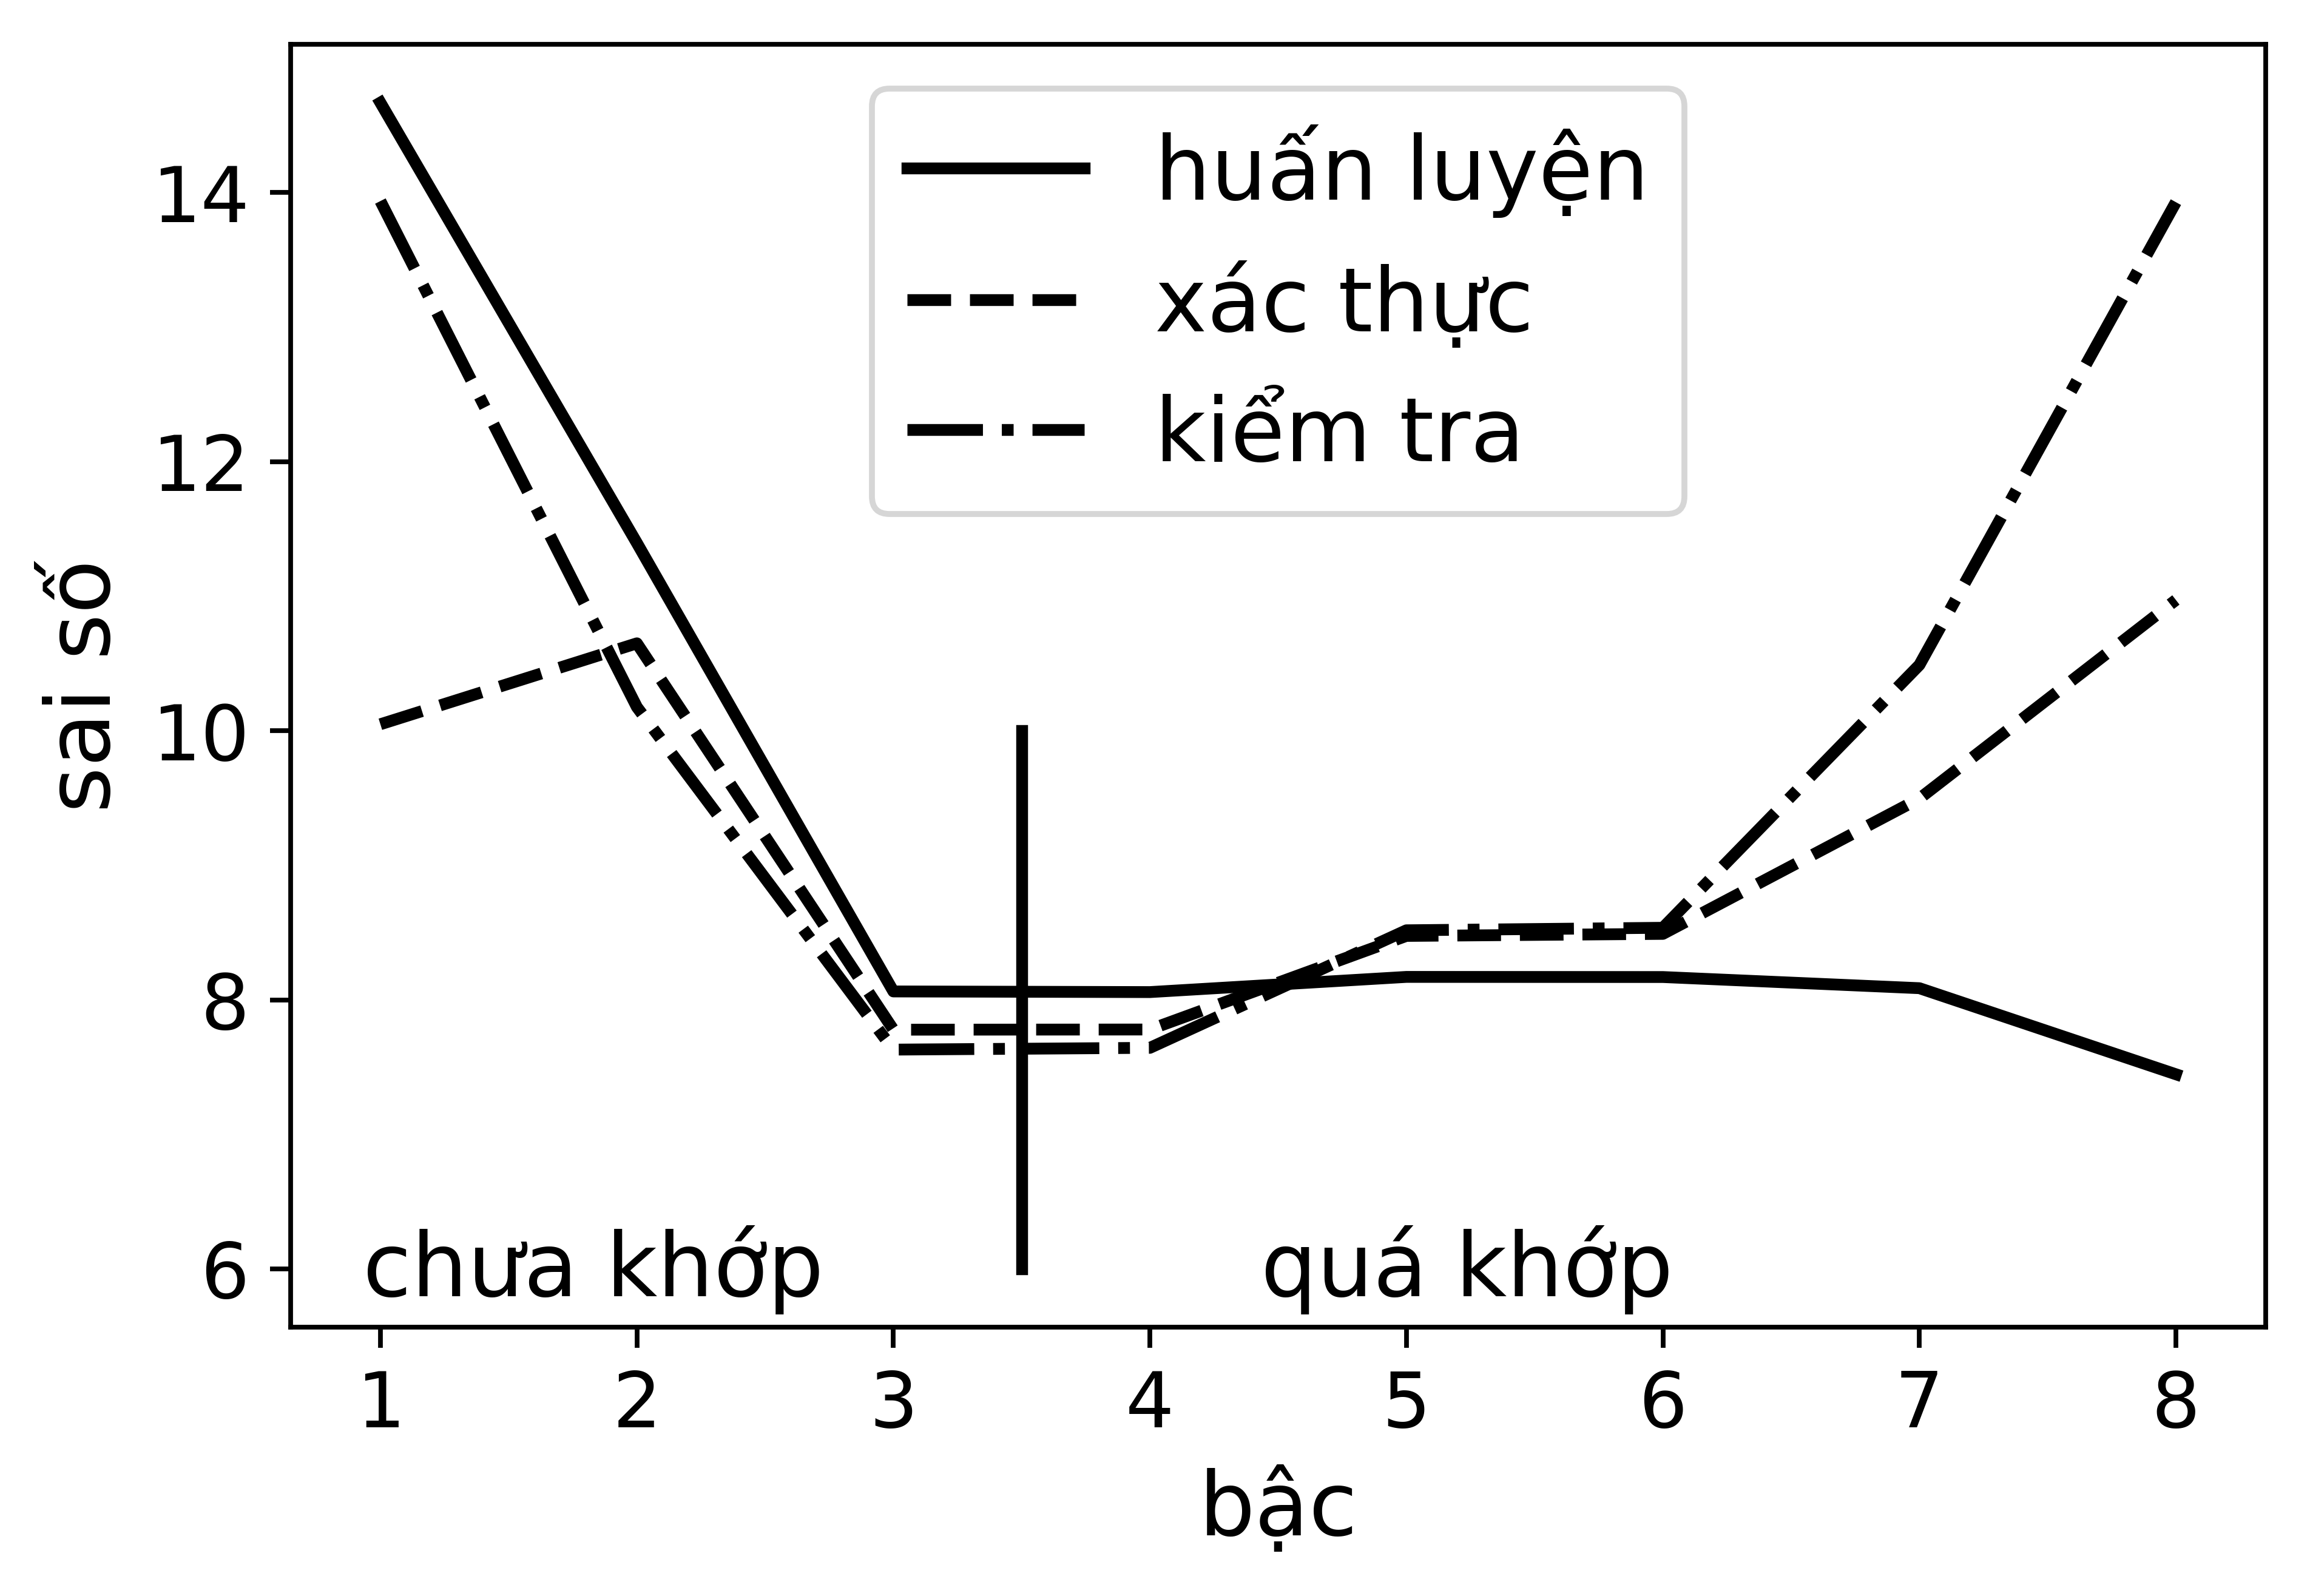
\includegraphics[width=.5\textwidth]{Chapters/01_Overview/15_overfitting/linreg_val.png}
}
\end{figure}
\index{tham số mô hình -- model parameter}
\index{model parameter -- tham số mô hình}
\index{siêu tham số mô hình -- model hyperparameter}
\index{model hyperparameter -- siêu tham số mô hình}
Hình~\ref{fig:15_validerror} mô tả ví dụ ở đầu chương với bậc của đa thức tăng
từ một đến tám. Tập xác thực là 10 điểm được lấy ra ngẫu nhiên từ tập huấn luyện
30 điểm ban đầu. Chúng ta hãy tạm chỉ xét hai đường nét liền và nét đứt, tương
ứng với {sai số huấn luyện} và {sai số xác thực}. Khi bậc của đa thức tăng lên,
{sai số huấn luyện} có xu hướng giảm. Điều này dễ hiểu vì đa thức bậc càng cao,
việc xấp xỉ càng chính xác. Quan sát đường nét đứt, khi bậc của đa thức là ba
hoặc bốn thì {sai số xác thực} thấp, sau đó nó tăng dần lên. Dựa vào
{sai số xác thực}, ta có thể xác định được bậc cần chọn là ba hoặc bốn. Quan
sát tiếp đường nét chấm gạch, tương ứng với {sai số kiểm tra}. Thật trùng hợp, sai số kiểm tra cũng đạt giá trị nhỏ nhất tại bậc bằng ba hoặc bốn và tăng lên khi bậc
tăng lên. Ở đây, kỹ thuật này đã tỏ ra hiệu quả. Mô hình phù hợp là mô hình có
bậc bằng ba hoặc bốn. Trong ví dụ này, tập xác thực đóng vai trò tìm ra bậc
của đa thức, tập huấn luyện đóng vai trò tìm các hệ số của đa thức
với bậc đã biết. Các hệ số của đa thức chính là các tham số mô hình,
trong khi bậc của đa thức có thể được coi là {siêu tham số}. Cả tập
huấn luyện và tập xác thực đều đóng vai trò xây dựng mô hình. Nhắc lại rằng
hai tập hợp này được tách ra từ tập huấn luyện ban đầu.

Trong ví dụ trên, ta vẫn thu được kết quả khả quan trên tập kiểm tra mặc dù không sử dụng tập này trong việc huấn luyện. Việc này xảy ra vì ta đã giả sử rằng dữ liệu xác thực và dữ liệu kiểm tra
có chung một đặc điểm nào đó (chung phân phối và đều chưa được mô hình nhìn thấy
khi huấn luyện).

Để ý rằng, khi bậc nhỏ bằng một hoặc hai, cả ba sai số đều cao, khi đó chưa khớp xảy ra.



\subsection{Xác thực chéo}
\label{ssec:crosvalid}
\index{xác thực -- validation!xác thực chéo -- cross-validation}
\index{validation -- xác thực!cross-validation -- xác thực chéo}
\index{xác thực -- validation!xác thực chéo k-fold}
\index{validation -- xác thực!xác thực chéo k-fold}
\index{xác thực -- validation!leave-one-out}
\index{validation -- xác thực!leave-one-out}

Trong nhiều trường hợp, lượng dữ liệu để xây dựng mô hình là hạn chế. Nếu lấy
quá nhiều dữ liệu huấn luyện ra làm dữ liệu xác thực, phần dữ liệu còn lại không
đủ để xây dựng mô hình. Lúc này, tập xác thực phải thật nhỏ để giữ được lượng dữ
liệu huấn luyện đủ lớn. Tuy nhiên, một vấn đề khác nảy sinh. Việc đánh giá trên tập xác thực quá nhỏ có thể gây ra hiện tượng thiên lệch. Có giải pháp nào cho tình huống này không?

Câu trả lời là \textit{xác thực chéo} ({cross-validation}).

Trong xác thực chéo, tập huấn luyện được chia thành $k$ tập con có kích thước gần bằng nhau và không giao nhau. Tại mỗi lần thử, một trong $k$ tập con đó được lấy ra làm tập xác thực, $k-1$ tập con còn lại được coi là tập huấn luyện. Như vậy, với mỗi bộ tham số mô hình, ta có $k$ mô hình khác nhau. Sai số huấn luyện và sai số xác thực được tính là trung bình cộng của các giá trị tương ứng trong $k$ mô hình đó. Cách làm này có tên gọi là \textit{xác thực chéo k-fold} (k-fold cross validation).

Khi $k$ bằng với số lượng phần tử trong tập huấn luyện ban đầu, tức mỗi
tập con có đúng một phần tử, ta gọi kỹ thuật này là \textit{leave-one-out}.

Thư viện scikit-learn hỗ trợ rất nhiều phương pháp phân chia dữ liệu để xây dựng mô hình. Bạn đọc có thể xem thêm
\textit{Cross-validation: evaluating estimator performance} (\url{https://goo.gl/Ars2cr}).





\section{Cơ chế kiểm soát}

\index{cơ chế kiểm soát -- regularization}
\index{regularization -- cơ chế kiểm soát}
Một nhược điểm lớn của xác thực chéo là số lượng mô hình cần huấn luyện tỉ lệ
thuận với $k$. Điều đáng nói là mô hình hồi quy đa thức như trên chỉ có một siêu
tham số liên quan đến độ phức tạp của mô hình cần xác định là bậc của đa thức.
Trong nhiều bài toán, lượng siêu tham số cần xác định thường lớn hơn, và
khoảng giá trị của mỗi tham số cũng rộng hơn, chưa kể có những
tham số có thể là số thực. Điều này dẫn đến việc huấn luyện nhiều mô hình là khó
khả thi. Có một kỹ thuật tránh quá khớp khác giúp giảm số mô hình cần huấn
luyện có tên là \textit{cơ chế kiểm soát} (regularization).

{Cơ chế kiểm soát} là một kỹ thuật phổ biến giúp tránh quá khớp theo hướng làm
giảm độ phức tạp của mô hình. Việc giảm độ phức tạp này có thể khiến lỗi huấn
luyện tăng lên nhưng lại làm tăng tính tổng quát của mô hình. Dưới đây là một
vài kỹ thuật kiểm soát.

\subsection{Kết thúc sớm}
\index{kết thúc sớm -- early stopping}
\index{early stopping -- kết thúc sớm}
Các mô hình machine learning phần lớn được xây dựng thông qua lặp đi lặp lại một
quy trình tới khi hàm mất mát hội tụ. Nhìn chung, giá trị hàm mất mát giảm dần
khi số vòng lặp tăng lên. Một giải pháp giúp giảm quá khớp là dừng thuật toán
trước khi nó hội tụ. Giải pháp này có tên là \textit{kết thúc sớm} (early stopping).

Vậy kết thúc khi nào là phù hợp? Kỹ thuật thường dùng là tách từ tập huấn luyện ra
một tập xác thực. Khi huấn luyện, ta tính toán cả sai số huấn luyện và sai số
xác thực, nếu sai số huấn luyện vẫn có xu hướng giảm nhưng sai số xác thực có xu
hướng tăng lên thì ta kết thúc thuật toán.

%  Sau một vòng lặp, ta tính cả \textit{sai số huấn luyện} và \textit{sai số xác thực}, đến khi \textit{sai số xác thực} có chiều hướng tăng lên thì dừng lại, và quay lại sử dụng mô hình tương ứng với điểm và \textit{sai số xác thực} đạt giá trị nhỏ.

% <div class="imgcap">
% <img src ="\assets\15_overfitting\EarlyStopping.png" align = "center" width = "400">
% <div class = "thecap">Hình 3: Early Stopping. Đường màu xanh là <i>sai số huấn luyện</i>, đường màu đỏ là <i>sai số xác thực</i>. Trục x là số lượng vòng lặp, trục y là error. Mô hình được xác định tại vòng lặp mà <i>sai số xác thực</i> đạt giá trị nhỏ nhất.  (<a href = "https://en.wikipedia.org/wiki/Overfitting">Overfitting - Wikipedia</a>).</div>
% </div>

\begin{figure}[t]
% caption on side
\floatbox[{\capbeside\thisfloatsetup{capbesideposition={right,top},capbesidewidth=6cm}}]{figure}[\FBwidth]
{\caption{
Kết thúc sớm. Thuật toán
huấn luyện dừng lại tại vòng lặp mà sai số xác thực đạt giá trị nhỏ nhất. }
\label{fig:15_earlystopping}}
{ % figure here
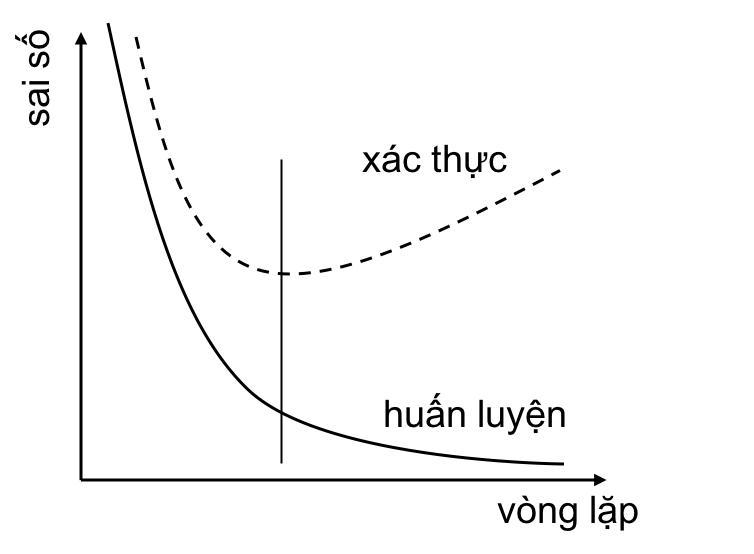
\includegraphics[width=.5\textwidth]{Chapters/01_Overview/15_overfitting/earlystopping_1.png}
}
\end{figure}


Hình~\ref{fig:15_earlystopping} mô tả cách tìm điểm \textit{kết thúc}. Chúng ta
thấy rằng phương pháp này tương tự phương pháp tìm bậc của đa thức ở đầu chương,
với độ phức tạp của mô hình có thể được coi là số vòng lặp cần chạy. Số vòng lặp
càng cao thì sai số huấn luyện càng nhỏ nhưng sai số xác thức có thể tăng lên, tức mô hình có khả năng bị quá khớp.


\subsection{Thêm số hạng vào hàm mất mát}
\index{tham số kiểm soát -- regularization parameter}
\index{regularization parameter -- tham số kiểm soát}
\index{hàm mất mát được kiểm soát -- regularized loss function}
\index{regularized loss function -- hàm mất mát được kiểm soát}
Kỹ thuật phổ biến hơn là thêm vào hàm mất mát một số hạng giúp
kiểm soát độ phức tạp mô hình. Số hạng này thường dùng để đánh giá độ phức tạp của
mô hình với giá trị lớn thể hiện mô hình phức tạp. {Hàm mất mát mới} được
gọi là \textit{hàm mất mát được kiểm soát} (regularized loss function), thường được định nghĩa như sau:
\begin{equation*}
\L_{\text{reg}}(\theta) = \L(\theta) + \lambda R(\theta)
\end{equation*}
Nhắc lại rằng $\theta$ được dùng để ký hiệu các tham số trong mô hình. $\L(\theta)$ là hàm mất mát phụ thuộc vào tập huấn luyện và $\theta$, $R(\theta)$ là số hạng kiểm soát chỉ phụ thuộc vào $\theta$. Số vô hướng $\lambda$ thường là một số dương nhỏ, còn được gọi là \textit{tham số kiểm soát} (regularization parameter).
Tham số kiểm soát thường được chọn là các giá trị nhỏ để đảm bảo nghiệm
của bài toán tối ưu $\L_{\text{reg}}(\theta)$ không quá xa nghiệm của bài toán
tối ưu $\L(\theta)$.

%  $\$
% Việc tối thiểu \textit{regularized loss function}, nói một cách tương đối, đồng nghĩa với việc tối thiểu cả \textit{loss function} và số hạng \textit{regularization}. Tôi dùng cụm "nói một cách tương đối" vì nghiệm của bài toán tối ưu \textit{loss function} và \textbf{regularized loss function} là khác nhau.  Chúng ta vẫn mong muốn rằng sự khác nhau này là nhỏ, vì vậy tham số regularization (\textit{regularizaton parameter}) $\lambda$ thường được chọn là một số nhỏ để biểu thức regularization không làm giảm quá nhiều chất lượng của nghiệm.

% Với các mô hình Neural Networks, một số kỹ thuật regularization thường được sử dụng là:

% Một vài hàm regularization thường được sử dụng được cho dưới đây:
\index{cơ chế kiểm soát -- regularization!kiểm soát $\ell_1$ -- $\ell_1$ regularization}
\index{regularization -- cơ chế kiểm soát!$\ell_1$ regularization -- kiểm soát $\ell_1$}
\index{cơ chế kiểm soát -- regularization!kiểm soát $\ell_2$ -- $\ell_2$ regularization}
\index{regularization -- cơ chế kiểm soát!$\ell_2$ regularization -- kiểm soát $\ell_2$}
\index{hồi quy ridge -- ridge regression}
\index{ridge regression -- hồi quy ridge}
\index{hồi quy lasso -- lasso regression}
\index{lasso regression -- hồi quy lasso}
\index{lựa chọn đặc trưng -- feature selection}
\index{feature selection -- lựa chọn đặc trưng}
% \index{sparsity}

Hai hàm kiểm soát phổ biến là $\ell_1$ norm và $\ell_2$ norm.
Ví dụ, khi chọn $R(\bw) = \|\bw\|_2^2$ cho hàm mất mát của hồi quy tuyến tính,
chúng ta sẽ thu được hồi quy ridge. Hàm kiểm soát $\ell_2$ này khiến các hệ số
trong $\bw$ không quá lớn, giúp tránh việc đầu ra phụ thuộc mạnh vào một
đặc trưng nào đó. Trong khi đó, nếu chọn $R(\bw) = \|\bw\|_1$, nghiệm $\bw$ tìm
được có xu hướng rất nhiều phần tử bằng không (\textit{nghiệm thưa}\footnote{\textit{L1 Norm Regularization and Sparsity Explained for
Dummies} (\url{https://goo.gl/VqPTLh}).}). Khi thêm kiểm soát $\ell_1$ vào
hàm mất mát của hồi quy tuyến tính, chúng ta thu được hồi quy LASSO. Các
thành phần khác không của $\bw$ tương đương với các đặc trưng quan trọng đóng
góp vào việc dự đoán đầu ra. Các đặc trưng ứng với thành phần bằng không của
$\bw$ được coi là ít quan trọng. Chính vì vậy, hồi quy LASSO cũng được coi là
một phương pháp giúp lựa chọn những đặc trưng hữu ích cho mô hình và có ý nghĩa trong việc trích chọn đặc trưng.

% \index{kháng nhiễu}
% \index{closed-form solution}
So với kiểm soát $\ell_2$, kiểm soát $\ell_1$ được cho là giúp mô hình kháng nhiễu tốt hơn. Tuy nhiên, hạn chế của kiểm soát $\ell_1$ là hàm $\ell_1$ norm không có đạo hàm mọi nơi, dẫn đến việc tìm nghiệm thường tốn thời gian hơn. Trong khi đó, đạo hàm của $\ell_2$ norm xác định mọi nơi. Hơn nữa, $\ell_2$ norm là một hàm lồi chặt, trong khi $\ell_1$ là một hàm lồi. Các tính chất của hàm lồi và hàm lồi chặt sẽ được thảo luận trong Phần~\ref{part:cvxopt}.


% \subsubsection{$l_2$ regularization}
% % Trong kỹ thuật này:
% \begin{equation*}
% R(\mathbf{w}) = \|\mathbf{w}\|_2^2
% \end{equation*}
% tức norm 2 của hệ số.
% \textit{Nếu bạn đọc chưa quen thuộc với khái niệm norm, bạn được khuyến khích đọc} \href{http://machinelearningcoban.com/math/#-norms-chuan}{phần phụ lục này}.

% Hàm số này có một vài đặc điểm đang lưu ý:

% \begin{itemize}
%     \item Thứ nhất, $\|\mathbf{w}\|_2^2$ là một hàm số \textit{rất mượt}, đạo hàm của nó đơn giản là $\mathbf{w}$, vì vậy đạo hàm của \textit{regularized loss function} cũng rất dễ tính, chúng ta có thể hoàn toàn dùng các phương pháp dựa trên gradient để cập nhật nghiệm. Cụ thể:
%     \begin{equation*}
%     \frac{\partial J_{\text{reg}} }{\partial \mathbf{w}} = \frac{\partial J}{\partial \mathbf{w}} + \lambda \mathbf{w}
%     \end{equation*}
%     \item Thứ hai, việc tối thiểu $\|\mathbf{w}\|_2^2$ đồng nghĩa với việc khiến cho các giá trị của hệ số $\mathbf{w}$ trở nên nhỏ gần với 0. Với Polynomial Regression, việc các hệ số này nhỏ có thể giúp các hệ số ứng với các số hạng bậc cao là nhỏ, giúp tránh overfitting. Với Multi-layer Pereceptron, việc các hệ số này nhỏ giúp cho nhiều hệ số trong các ma trận trọng số là nhỏ. Điều này tương ứng với việc số lượng các hidden units \textit{hoạt động} (khác không) là nhỏ, cũng giúp cho MLP tránh được hiện tượng overfitting.
% \end{itemize}

% $l_2$ regularization là kỹ thuật được sử dụng nhiều nhất để giúp Neural Networks tránh được overfitting. Nó còn có tên gọi khác là \textbf{weight decay}. \textit{Decay} có nghĩa là \textit{tiêu biến}.

% Trong Xác suất thống kê, Linear Regression với $l_2$ regularization được gọi là \href{https://en.wikipedia.org/wiki/Tikhonov_regularization}{\textbf{Ridge Regression}}. Hàm mất mát của \textit{Ridge Regression} có dạng:
% \begin{equation*}
% J(\mathbf{w}) = \frac{1}{2} \|\mathbf{y} - \mathbf{Xw}\|_2^2 + \lambda \|\mathbf{w}\|_2^2
% \end{equation*}
% trong đó, số hạng đầu tiên ở vế phải chính là hàm mất mát của Linear Regression. Số hạng thứ hai chính là phần regularization.


% \subsection{Tikhonov regularization}
% \begin{equation*}
% \lambda R(\mathbf{w}) = \|\Gamma \mathbf{w}\|_2^2
% \end{equation*}

% Với $\Gamma$ (viết hoa của gamma) là một ma trận. Ma trận $\Gamma$ hay được dùng nhất là ma trận đường chéo. Nhận thấy rằng $l_2$ regularization chính là một trường hợp đặc biệt của Tikhonov regularization với $\Gamma = \lambda \mathbf{I}$ với $\mathbf{I}$ là ma trận đơn vị (\textit{the identity matrix}), tức các phần tử trên đường chéo của $\Gamma$ là như nhau.

% Khi các phần tử trên đường chéo của $\Gamma$ là khác nhau, ta có một phiên bản gọi là \textit{weighted $l_2$ regularization}, tức đánh trọng số khác nhau cho mỗi phần tử trong $\mathbf{w}$. Phần tử nào càng bị đánh trọng số cao thì nghiệm tương ứng càng nhỏ (để đảm bảo rằng hàm mất mát là nhỏ). Với Polynomial Regression, các phần tử ứng với hệ số bậc cao sẽ được đánh trọng số cao hơn, khiến cho xác suất để chúng gần 0 là lớn hơn.


% \subsection{Regularizers for sparsity}

% Trong nhiều trường hợp, ta muốn các hệ số \textit{thực sự} bằng 0 chứ không phải là \textit{nhỏ gần 0} như $l_2$ regularization đã làm phía trên. Lúc đó, có một regularization khác được sử dụng, đó là $l_0$ regularization:
% \begin{equation*}
% R(\mathbf{W}) = \|\mathbf{w}\|_0
% \end{equation*}

% Norm 0 không phải là một norm thực sự mà là giả norm. (Bạn được khuyến khích đọc thêm về \href{http://machinelearningcoban.com/math/#-norms-chuan}{norms (chuẩn)}). Norm 0 của một vector là số các phần tử khác không của vector đó. Khi norm 0 nhỏ, tức rất nhiều phần tử trong vector đó bằng 0, ta nói vector đó là \textit{sparse}.

% Việc giải bài toán tổi thiểu norm 0 nhìn chung là khó vì hàm số này không \textit{convex}, không liên tục. Thay vào đó, norm 1 thường được sử dụng:
% \begin{equation*}
% R(\mathbf{W}) = \|\mathbf{w}\|_1 = \sum_{i=0}^d \|w_i\|
% \end{equation*}

% Norm 1 là tổng các trị tuyệt đối của tất cả các phần tử. Người ta đã chứng minh được rằng tối thiểu norm 1 sẽ dẫn tới nghiệm có nhiều phần tử bằng 0. Ngoài ra, vì norm 1 là một \textit{norm thực sự} (proper norm) nên hàm số này là \textit{convex}, và hiển nhiên là liên tục, việc giải bài toán này dễ hơn việc giải bài toán tổi thiểu norm 0. Về $l_1$ regularization, bạn đọc có thể đọc thêm trong \href{http://machinelearningcoban.com$l_1$ regularization}{lecture note} này. Việc giải bài toán $l_1$ regularization nằm ngoài mục đích của tôi trong bài viết này. Tôi hứa sẽ quay lại phần này sau. (Vì đây là phần chính trong nghiên cứu của tôi).

% Trong Thống Kê, việc sử dụng $l_1$ regularization còn được gọi là \href{https://en.wikipedia.org/wiki/Lasso_(statistics}{LASSO}) (Least Absolute Shrinkage and Selection Operator)).

% Khi cả $l_2$ và $l_1$ regularization được sử dụng, ta có mô hình gọi là \href{https://en.wikipedia.org/wiki/Elastic_net_regularization}{Elastic Net Regression}.


% \subsection{Regularization trong sklearn}

% Trong \href{http://scikit-learn.org/stable/modules/generated/sklearn.linear_model.LogisticRegression.html}{sklearn}, ví dụ \href{http://machinelearningcoban.com/2017/01/27/logisticregression/}{Logistic Regression}, bạn cũng có thể sử dụng các $l_1$ và $l_2$ regularizations bằng cách khai báo biến \pythoninline{penalty='l1'} hoặc \pythoninline{penalty = 'l2'} và biến \pythoninline{C}, trong đó \pythoninline{C} là \textit{nghịch đảo} của $\lambda$. Trong các bài trước khi chưa nói về  Overfitting và Regularization, tôi có sử dụng \pythoninline{C = 1e5} để chỉ ra rằng $\lambda$ là một số rất nhỏ.


% \section{Các phương pháp khác}
% Ngoài các phương pháp đã nêu ở trên, với mỗi mô hình, nhiều phương pháp tránh overfitting khác cũng được sử dụng. Điển hình là \href{http://jmlr.org/papers/volume15/srivastava14a/srivastava14a.pdf}{Dropout trong Deep Neural Networks mới được đề xuất gần đây}. Một cách ngắn gọn, dropout là một phương pháp \textit{tắt} ngẫu nhiên các units trong Networks. \textit{Tắt} tức cho các unit giá trị bằng không và tính toán feedforward và backpropagation bình thường trong khi training. Việc này không những giúp lượng tính toán giảm đi mà còn làm giảm việc overffitng. Tôi xin được quay lại vấn đề này nếu có dịp nói  sâu về Deep Learning trong tương lai.

% Bạn đọc có thể tìm đọc thêm với các từ khóa: \href{https://en.wikipedia.org/wiki/Pruning_(decision_trees}{pruning}) (tránh overftting trong Decision Trees), \href{https://en.wikipedia.org/wiki/VC_dimension}{VC dimension} (đo độ phức tạp của mô hình, độ phức tạp càng lớn thì càng dễ bị overfitting).


% \section{Tóm tắt và thảo luận}

% \subsection{bias variance tradeoff}

% \begin{itemize}
%     \item Một mô hình mô tốt là mộ mô hình có \textit{tính tổng quát}, tức mô tả
%     được dữ liệu cả trong lẫn ngoài tập huấn luyện. Mô hình chỉ mô tả tốt dữ
%     liệu trong tập huấn luyện được gọi là \textbf{overfitting}.

%     \item Để tránh overfitting, có rất nhiều kỹ thuật được sử dụng, điển hình là \textbf{cross-validation} và \textbf{regularization}. Trong Neural Networks, \textbf{weight decay} và \textbf{dropout} thường được dùng.
% \end{itemize}
\index{suy giảm trọng số -- weight decay}
\index{weight decay -- suy giảm trọng số}
Trong mạng neuron, phương pháp sử dụng kiểm soát $\ell_2$ còn được gọi là \textit{suy giảm trọng số} (weight decay)~\cite{krogh1992simple}. Ngoài ra, gần đây có một phương pháp kiểm soát rất hiệu quả cho các mạng neuron sâu được sử dụng là \textit{dropout}~\cite{srivastava2014dropout}.

\section{Đọc thêm}
\begin{enumerate}
\item A. Krogh \etal, \textit{A simple weight decay can improve generalization.} NIPS 1991~\cite{krogh1992simple}.

\item N. Srivastava \etal, \textit{Dropout: A Simple Way to Prevent Neural
Networks from  Overfitting}, Journal of Machine Learning Research 15.1
(2014): 1929-1958~\cite{srivastava2014dropout}.

\item \textit{Understanding the Bias-Variance Tradeoff} (\url{https://goo.gl/yvQv3w}).

\end{enumerate}
